\documentclass[a4paper]{article}

\usepackage[utf8]{inputenc}
\usepackage[T1]{fontenc}
\pagenumbering{arabic}
\usepackage[spanish]{babel}
\renewcommand\spanishtablename{Tabla}
\usepackage{a4wide}
\usepackage{amsmath}
\usepackage{amssymb,amsfonts,textcomp}
\usepackage{color}
\usepackage{array}
\usepackage{supertabular}
\usepackage{hhline}
\usepackage{hyperref}
\usepackage{fancyhdr}
%\usepackage{showframe}
\usepackage{longtable}
\usepackage[table]{xcolor}
%\usepackage{showframe }
%\hypersetup{pdftex, colorlinks=true, linkcolor=blue, citecolor=blue, filecolor=blue, urlcolor=blue, pdftitle=, pdfauthor=, pdfsubject=, pdfkeywords=}
\usepackage[pdftex]{graphicx}
% footnotes configuration
\makeatletter
\renewcommand\thefootnote{\arabic{footnote}}
\makeatother
% Text styles
\newcommand\textstyleStrongEmphasis[1]{\textbf{#1}}
% Outline numbering
\setcounter{secnumdepth}{0}
\makeatletter
\newcommand\arraybslash{\let\\\@arraycr}
\makeatother
% List styles
\newcommand\liststyleWWNumxxix{%
\renewcommand\labelitemi{{}-}
\renewcommand\labelitemii{o}
\renewcommand\labelitemiii{[F0A7?]}
\renewcommand\labelitemiv{[F0B7?]}
}
\newcommand\liststyleLi{%
\renewcommand\labelitemi{{\textbullet}}
\renewcommand\labelitemii{${\circ}$}%
\renewcommand\labelitemiii{${\blacksquare}$}
\renewcommand\labelitemiv{{\textbullet}}
}
\newcommand\liststyleLii{%
\renewcommand\labelitemi{{\textbullet}}
\renewcommand\labelitemii{${\circ}$}
\renewcommand\labelitemiii{${\blacksquare}$}
\renewcommand\labelitemiv{{\textbullet}}
}
\newcommand\liststyleLiii{%
\renewcommand\labelitemi{{\textbullet}}
\renewcommand\labelitemii{${\circ}$}
\renewcommand\labelitemiii{${\blacksquare}$}
\renewcommand\labelitemiv{{\textbullet}}
}
\newcommand\liststyleLiv{%
\renewcommand\labelitemi{{\textbullet}}
\renewcommand\labelitemii{${\circ}$}
\renewcommand\labelitemiii{${\blacksquare}$}
\renewcommand\labelitemiv{{\textbullet}}
}
\newcommand\liststyleLv{%
\renewcommand\labelitemi{{\textbullet}}
\renewcommand\labelitemii{${\circ}$}
\renewcommand\labelitemiii{${\blacksquare}$}
\renewcommand\labelitemiv{{\textbullet}}
}
\newcommand\liststyleLvi{%
\renewcommand\labelitemi{{\textbullet}}
\renewcommand\labelitemii{${\circ}$}
\renewcommand\labelitemiii{${\blacksquare}$}
\renewcommand\labelitemiv{{\textbullet}}
}
\newcommand\liststyleLvii{%
\renewcommand\labelitemi{{\textbullet}}
\renewcommand\labelitemii{{\textbullet}}
\renewcommand\labelitemiii{{\textbullet}}
\renewcommand\labelitemiv{{\textbullet}}
}
\newcommand\liststyleLviii{%
\renewcommand\labelitemi{{\textbullet}}
\renewcommand\labelitemii{{\textbullet}}
\renewcommand\labelitemiii{{\textbullet}}
\renewcommand\labelitemiv{{\textbullet}}
}
\newcommand\liststyleLix{%
\renewcommand\labelitemi{{\textbullet}}
\renewcommand\labelitemii{{\textbullet}}
\renewcommand\labelitemiii{{\textbullet}}
\renewcommand\labelitemiv{{\textbullet}}
}
\newcommand\liststyleLx{%
\renewcommand\labelitemi{{\textbullet}}
\renewcommand\labelitemii{{\textbullet}}
\renewcommand\labelitemiii{{\textbullet}}
\renewcommand\labelitemiv{{\textbullet}}
}
% Page layout (geometry)
\setlength\voffset{-1in}
\setlength\hoffset{-1in}
\setlength\topmargin{2cm}
\setlength\oddsidemargin{2cm}
%\setlength\textheight{24.203001cm}
\setlength\textwidth{17.001cm}
%\setlength\footskip{0.0cm}
%\setlength\headheight{0.998cm}
%\setlength\headsep{0.499cm}
% Footnote rule
\setlength{\skip\footins}{0.119cm}
\renewcommand\footnoterule{\vspace*{-0.018cm}\setlength\leftskip{0pt}\setlength\rightskip{0pt plus 1fil}\noindent\textcolor{black}{\rule{0.25\columnwidth}{0.018cm}}\vspace*{0.101cm}}
% Pages styles
\makeatletter
\newcommand\ps@Standard{
  \renewcommand\@oddhead{[Warning: Draw object ignored]}
  \renewcommand\@evenhead{\@oddhead}
  \renewcommand\@oddfoot{}
  \renewcommand\@evenfoot{}
  \renewcommand\thepage{\arabic{page}}
}
\newcommand\ps@FirstPage{
  \renewcommand\@oddhead{}
  \renewcommand\@evenhead{}
  \renewcommand\@oddfoot{}
  \renewcommand\@evenfoot{}
  \renewcommand\thepage{\arabic{page}}
}
\makeatother

\setlength\tabcolsep{1mm}
\renewcommand\arraystretch{1.3}
\title{}
\author{}
\date{2013-06-03}

\renewcommand{\baselinestretch}{1.2}

\begin{document}

\pagestyle{empty}
\setcounter{page}{0}


\includegraphics[width=3cm]{logo-uclm.jpg}
\hfill

\includegraphics[width=3cm]{logo-esii.png}

{\centering \par}
\begin{center}

\includegraphics[width=2.96cm,height=3.522cm]{logo-conciti.png}
\end{center}

\vskip 3em
{\centering\bfseries\large
UNIVERSIDAD DE CASTILLA-LA MANCHA
\par}

\vskip 3em
{\centering\bfseries\large
ESCUELA SUPERIOR DE INFORMÁTICA
\par}

{\centering\bfseries\large
Departamento de Sistemas Informáticos\footnote{DEPARTAMENTO DE SISTEMAS INFORMÁTICOS o DEPARTAMENTO DE
INGENIERÍA ELÉCTRICA, ELECTRÓNICA, AUTOMÁTICA Y COMUNICACIONES o DEPARTAMENTO DE MATEMÁTICAS o cualquier otro
de la UCLM al que pertenezca el director. \par }
\par}

\vskip 3em
{\centering\bfseries\large
ANTEPROYECTO DEL TRABAJO FIN DE GRADO
\par}

{\centering\bfseries\large
GRADO EN INGENIERÍA INFORMÁTICA
\par}

{\centering\bfseries\large
TECNOLOGÍA ESPECÍFICA DE / INTENSIFICACIÓN / ITINERARIO DE \footnote{INGENIER\'IA DEL SOFTWARE o INGENIER\'IA DE COMPUTADORES o COMPUTACI\'ON o
TECNOLOG\'IAS DE LA INFORMACI\'ON (esta \'ultima est\'a tambi\'en asociada a los TFG del \textbf{curso} de
\textbf{adaptaci\'on})}
\par}

\vskip 3em
{\centering\bfseries
(Título del TFG)
\par}

\vfill % Rellena espacio automáticamente hasta ajustar al margen inferior 

Autor: Fernando Luján Martínez

Director: Gregorio Díaz Descalzo
\footnote{Sólo en el caso de que haya un segundo director.} (nombre y apellidos)

\vskip 1em 
\mbox{\begin{minipage}[b][2.5cm][c]{0.7\linewidth} {\large Mes, 2018}  \end{minipage}}
\hfill % Rellena espacio automáticamente hasta que la image se ajuste a la derecha
\mbox{
\includegraphics[width=2.5cm]{logo-euroinf.png}}
\vskip 1em %Un línea en blanco para que el logo de Euroinf no se pegue al footnote

\clearpage\pagestyle{plain}
\pagenumbering{roman}

\setcounter{tocdepth}{10}
\renewcommand\contentsname{\'Indice de contenido}
\tableofcontents

\clearpage
%\pagestyle{empty}
\liststyleWWNumxxix

\clearpage\pagestyle{plain}
\pagenumbering{arabic}
\setcounter{page}{1}

\section{1.\ INTRODUCCI\'ON}

En la actualidad vivimos inmersos en un mundo que genera ingentes cantidades de información, cualquier sistema por simple que sea genera una gran cantidad de datos. Poder analizar todo lo que se genera para obtener información relevante es uno de los objetivos que se persiguen. Esto se puede hacer de diferentes formas. Una de las posibles opciones es el Big Data, este concepto implica guardar los datos para mas adelante analizarlos \cite{libroBigData}. Este procedimiento tiene una serie de ventajas y desventajas. Algunas de estos inconvenientes son la necesidad de (mucho) espacio de  almacenamiento, la información guardada puede no ser tan valiosa como se pensaba o los resultados del análisis no sean inmediatos y hasta que no tengamos suficientes datos no podremos llegar a ninguna conclusión.

Para evitar las desventajas comentadas, principalmente la tercera, donde en ciertos sectores, como pueden ser los industriales, es imprescindible tener conocimiento al instante del estado en el que se encuentran los sistemas. De esta necesidad nace CEP (complex event processing), definido como un conjunto de técnicas y herramientas para analizar y controlar una serie de eventos complejos interrelacionados. Sin embargo, para comprender mejor el concepto de CEP debemos definir, claramente que es un evento complejo, el cual es un evento que que solo puede suceder si otra serie de eventos, que llamaremos simples, han sucedido y se ha detectado una relación entre ellos, esta puede ser temporal o causal \cite{libro introduccion cep}. De esta forma no es necesario el almacenamiento de todos datos obtenidos, solo el de los eventos simples deseados. Por otro lado, otra de las ventajas de CEP es que los resultados de los análisis están disponibles conforme se generan y detectan los eventos, listos para la toma de decisiones.

CEP también es muy útil en entornos complicados en lo que no es posible tener un extenso almacenamiento, la conexión para la transferencia de datos no tiene un gran ancho de banda, la velocidad o la fiabilidad en la entrega de todos los paquetes no es la mejor.

Pero, ¿en qué entorno aplicaremos el concepto de CEP?, en el de las plantas fotovoltaicas. Sin embargo, para poder tratar con un entorno real, con datos y eventos reales hemos decidido ir de la mano de Ingeteam, empresa especializada en conversión de energía, la cual desarrolla equipos electrónicos de potencia y de control, generadores, motores bombas y proyectos de ingeniería eléctrica y de automatización \cite{webIngeteam}. Esta compañía, con oficinas en Albacete, tiene acceso a plantas fotovoltaicas donde tienen instalados algunos de los equipos comentados.

En el caso en que nos centraremos, análisis de datos obtenidos desde plantas fotovoltaicas, esta claro que todo lo indicado arriba se cumple:

\begin{itemize}
\item Normalmente las plantas fotovoltaicas están ubicadas lejos de núcleos urbanos grandes, por esto la conexión hacia el exterior (internet) no es idónea, ya sea por la poca banda ancha, perdidas de paquetes o poca velocidad de transferencia.
\item Poner un sistema, en cada una de las plantas, que almacene y examine los datos tampoco es interesante en términos de mantenimiento y por tanto económicos.
\item Aunque la extensión de una de estas plantas es variable, suelen ser de al menos unas hectáreas. Por tanto si estamos tratando de detectar fallos en alguno de los componentes, ir componente por componente sería inviable.
\item Por último, incluso obviando lo anterior y siendo capaces de almacenar y analizar los datos en cada una de las plantas, si algo esta dañado cuando interesa saberlo es lo antes posible, algo que con CEP podemos conseguir, y no pasado un tiempo, como sucede con Big Data. Añadiendo a todo esto el potencial de detectar eventos por muy complejos que sean.
\end{itemize}

\begin{figure}[ht]
    \centering
    {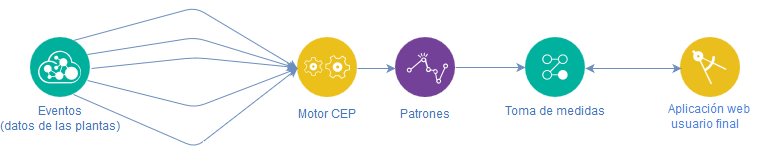
\includegraphics[width=150mm]{vision_general_fase_3.png}}
    \caption{esquema general para comprender mejor el objetivo que persigue el proyecto.}
    \label{fig:mesh1}
\end{figure}

En este Trabajo Fin de Grado lo que trataremos es, de la mano de Ingeteam, desarrollar un sistema capaz de detectar eventos simples y lo que es más interesante reconocer patrones de eventos (eventos complejos).

En líneas generales, tendremos una serie de datos que llegarán de los campos solares, estos datos serán los llamados eventos simples. Toda esta información se filtrará y acondicionará para el motor CEP donde estarán incluidos los patrones de eventos que desarrollaremos. Cuando el motor detecte a partir de los eventos que ha recibido un patrón se tomarán una serie de medidas, como puede ser el envío de una alerta a un técnico. Esto lo podemos ver gráficamente en la figura \ref{fig:mesh1}.

\section{2. TECNOLOG\'IA ESPEC\'IFICA / INTENSIFICACIÓN / ITINERARIO CURSADO POR EL ALUMNO}

\bigskip
En esta sección adjunto dos tablas. La primera hace referencia a la tecnología del grado que escogí, Tabla \ref{tab:tablaTecnologia}, en la primera columna aparecen todas las tecnologías disponibles en el grado y en la segunda marcada con la letra x mi opción. La segunda esta relacionada con todas las competencias que incluye la tecnología por la que opté, teniendo en la primera columna la competencia y en la segunda la justificación de la misma, Tabla \ref{tab:tablaCompetencias}.

\clearpage\pagestyle{plain}
%\thispagestyle{FirstPage}

\begin{longtable}{m{6.803cm} m{2.605cm}}
    \iffalse
    	primera fila, cabecera
    \fi
    \rowcolor{gray!50}
	{\color{black} \textbf{Marcar la Tecnolog\'ia Cursada}} &
	{\color{black} \textbf{Selección}}\\\hline
	
    {\color{black} \textbf{Tecnolog\'ias de la Informaci\'on}} &
    {\color{black} \textbf{}}\\\hline
	\rowcolor{gray!30}
    {\color{black} \textbf{Computaci\'on}}&
    {\color{black} \textbf{}}\\\hline
	
    {\color{black} \textbf{Ingenier\'ia del Software}}&
    {\color{black} \textbf{X}}\\\hline
	\rowcolor{gray!30}

	{\color{black} \textbf{Ingenier\'ia de Computadores}}&
    {\color{black} \textbf{}}\\\hline
\caption{tecnolog\'ia Espec\'ifica cursada por el alumno}\label{tab:tablaTecnologia}
\end{longtable}

\bigskip
\begin{longtable}{m{5.605cm}m{10.849cm}}
  	\iffalse
    	primera fila, cabecera
    \fi
    \rowcolor{gray!50}
	{\color{black} \textbf{Competencias}} &
	{\color{black} \textbf{Justificaci\'on}}\\\hline
    
    {\color{black} Competencia 1: capacidad para desarrollar, mantener y evaluar servicios y sistemas software que satisfagan todos los requisitos del usuario y se comporten de forma fiable y eficiente, sean asequibles de desarrollar y mantener y cumplan normas de calidad, aplicando las teor\'ias, principios, m\'etodos y pr\'acticas de la Ingenier\'ia del Software.} &
    {\color{black} La justificación de esta competencia la desmigaré en cuatro partes.
    {\begin{itemize} 
    \item Primero, la metodología de desarrollo que utilizaré será scrum junto con prototipado.
    \item Segundo, las tecnologías utilizadas serán, principalmente, el lenguaje Esper EPL y su motor CEP. Aunque esta tecnología es la piedra angular de este desarrollo, de forma secundaria necesitamos más herramientas que le provean los datos, que manejen las salidas del motor y que den cohesión al proyecto. Por esto también utilizaremos la plataforma Anypoint de MuleSoft, la cual es un ESB (Enterprise service bus). Este ESB esta formado por flujos los cuales se pueden configurar con diferentes módulos conectables.
    \item Tercero, el mantenimiento del software es algo fundamental pero debido a la naturaleza del producto que vamos desarrollar, a priori, no habrá un proceso de mantenimiento como tal. Tanto la documentación como el código y su configuración estarán formados teniendo siempre en mente que este código será leído y modificado por alguien diferente a mi.
    \item Por último, para evaluar el proyecto desde el principio se aplicarán pruebas unitarias y pruebas de integración además de reuniones periódicas en las que se tendrán pruebas de aceptación por parte de Ingeteam.
    \end{itemize}}
    }\\
    
    \rowcolor{gray!30}
    {\color{black} Competencia 2: Capacidad para valorar las necesidades del cliente y especificar los requisitos software para satisfacer estas necesidades, reconciliando objetivos en conflicto mediante la b\'usqueda de compromisos aceptables dentro de las limitaciones derivadas del coste, del tiempo, de la existencia de sistemas ya desarrollados y de las propias organizaciones.} &
    {\color{black} Para la toma de requisitos al cliente y más adelante para que todo encaje, se harán reuniones periódicas al principio y al final de cada iteración (y siempre que se precisen).
    La elicitación de los requisitos se hará con historias de usuario por un lado, para la parte más relacionada con la sección del sistema cercano al usuario final. Esto es así porque del resto de posibilidades que nos quedan, como pueden ser los casos de uso, no son lo más adecuado a la metodología que vamos a utilizar. Por otro lado, para recoger los patrones utilizaremos el storyboards.\newline
    Finalmente, para dejar claro que lo realizado en las iteraciones se ajusta a lo definido inicialmente cada historia de usuario tendrá una prueba de aceptación, relativa al prototipo que se entregue.}\\
    
    {\color{black} Competencia 3: Capacidad de dar soluci\'on a problemas de integraci\'on en funci\'on de las estrategias, est\'andares y tecnolog\'ias disponibles. } &
    {\color{black} 
    La integración del sistema dentro del entorno real será en un servidor de la empresa (propio o contratado) donde se ejecutará el software de creado. Todas las tecnologías que vayan a ser utilizadas, inicialmente, serán analizadas para comprobar que serán compatibles con el entorno final.}\\
    
    \rowcolor{gray!30}
    {\color{black} Competencia 4: Capacidad de identificar y analizar problemas y dise\~nar, desarrollar, implementar, verificar y documentar soluciones software sobre la base de un conocimiento adecuado de las teor\'ias, modelos y t\'ecnicas actuales.} &
    {\color{black}El problema que vamos a atacar es detectar ciertos desgastes y futuros fallos en todo el sistema que hay detrás de una o varias plantas fotovoltaicas. Para ello vamos a analizar todos los datos generados de las placas de estos campos. Al ser una gran cantidad, el monitóreo de las instalaciones debe de ser en tiempo real, los resultados del análisis de los datos deben de estar lo antes posible y por último inferir, a priori, los datos para obtener esos resultados no es una tarea trivial, por tanto podemos decir que la opción que mejor se ajusta a estos requisitos es CEP.
    
    Todo esto es relativo al tema de la tecnología que, según nuestra perspectiva, mejor se podría ajustar al problema que estamos tratando. Pero por muy acertado que sea CEP, como sabemos, es necesario llevar a cabo un proceso de desarrollo válido y coherente. Por esto, la elicitación de requisitos (storyboards, historias de usuario y lenguaje natural), la implementación (y entregas de artefactos) y, por último, las pruebas deben de estar bien ajustadas al contexto que rodea a este proyecto.}\\
    
    {\color{black} Competencia 5: Capacidad de identificar, evaluar y gestionar los riesgos potenciales asociados que pudieran presentarse.} &
    {\color{black} Como ya comentamos para el problema principal que tratamos de solucionar CEP encaja perfectamente.
      Como el sistema a desarrollar esta formado por sistemas dispares, debemos de ser capaces de hacerlos coexistir. Esto lo podemos hacer nosotros mismos o mediante el esb, con el cual conseguimos que todo este proceso se simplifique infinitamente. Por eso se ha decidido utilizar uno.
      Por otro lado la metodología por la que hemos optado es la que mejor se ajusta todos los contratiempos que vamos a tener.
   	}\\
    
    \rowcolor{gray!30}
    {\color{black} Competencia 6: Capacidad para dise\~nar soluciones apropiadas en uno o m\'as dominios de aplicaci\'on utilizando m\'etodos de la ingenier\'ia del software que integren aspectos \'eticos, sociales, legales y econ\'omicos.} &
    {\color{black} Para poder llevar a buen puerto este proyecto y que alcance los objetivos que nos hemos planteado es preciso diseñar una una hoja de ruta, una planificación, que nos asegure este propósito. Para ello teniendo en cuenta todos los condicionantes que nos rodean, la opción que creemos mas viable es definir en tres grandes iteraciones o fases el proyecto. Cada una de ella estará a su vez dividida en varios springs mas cortos, de una semana. La primera fase, relacionada con la toma y elicitación de requisitos y diseño. La segunda ya incluye implementación, testeo y entrega de un primer prototipo capaz de detectar patrones y notificarlos a a partir de datos ya recolectados y almacenados. La tercera fase incluirá una revisión de patrones, pudiendo añadir alguno nuevo; y se desarrollará el adaptador para que los datos finalmente provengan en tiempo real, saliendo de esta última iteración la entrega definitiva.
    }\\
\caption{tecnolog\'ia Espec\'ifica cursada por el alumno}\label{tab:tablaCompetencias}
\end{longtable}
\bigskip

\section{3. \ OBJETIVOS}
Siendo concisos, el objetivo principal de este trabajo es conseguir analizar una serie de datos, obtenidos de una serie de plantas fotovoltaicas, en tiempo real para obtener una serie de alertas, recomendaciones o acciones. De esta forma subsanar fallos o averías, pero no solo en el presente sino también predecirlas en el futuro.

Esto se puede dividir en 4 sub-objetivos, los cuales son:

\begin{itemize}
	\item Creación de un adaptador al flujo de datos que nos proporcione Ingeteam (librería de java poi). \newline
    \textbf{Limitaciones y condicionantes:} en este sub-objetivo tenemos una limitación importante y es que por parte de ingeteam, no todas las plantas nos pueden proporcionar los datos en tiempo real ya que algunas de ellas no son ellos los propietarios.\newline 
    \textbf{Sobre la tecnología:} esta mas que probada y lleva ya bastantes años en funcionamiento con una gran documentación y comunidad detrás.
    
    \item Obtención, diseño e implementación de patrones complejos. \newline
    \textbf{Limitaciones y condicionantes:} los datos que emanan de las plantas en algunos casos no es trivial su análisis, es decir, detectar que datos, de forma conjunta e interrelacionado de una manera especifica, podrían ser un patrón interesante. La solución a esto pasa casi por la prueba y error. (Una de las razones por las que se ha decidido utilizar scrum y prototipado). \newline
    \textbf{Sobre la tecnología:} para el diseño no será necesaria ninguna tecnología especifica pero para su implementación si que deberemos de hacer uso del ya mencionado Esper EPL, siendo este una de las mejores opciones como comentamos mas adelante en el listado de sus ventajas. \newline
    
    \item Crear las respuestas a los patrones detectados. \newline
    \textbf{Limitaciones y condicionantes:} aunque es un objetivo que debemos de alcanzar, el como no esta definido completamente, en otras palabras, Ingeteam debe de definirnos las acciones y objetivos que desean alcanzar con los patrones detectados. Inicialmente nos comentaron de insertar en su base de datos de alertas. Hasta donde sabemos la base de datos es MySQL, cuya configuración por nuestra parte no debe de ser complicada gracias a enorme cantidad de tutoriales y documentación.\newline
    
    \item Integración de todos los sistemas necesarios.\newline
    \textbf{Limitaciones y condicionantes:} en un principio esta es la parte que esta mejor definida está, las pruebas que se han hecho con el ESB parecen bastante satisfactorias. Evidentemente, aunque aun no hemos tenido problemas, es el paso mas crítico ya que debe de aunar una gran cantidad de lenguajes, librerías, el motor CEP y conexiones a sistemas externos.\newline
    \textbf{Sobre la tecnología:} para llevar a cabo esto utilizaremos Anypoint Studio junto con mule, con los que no hemos tenido problema alguno creando flujos de datos.

\end{itemize}
 

\section[4. M\'ETODO Y FASES DE TRABAJO]{4. M\'ETODO Y FASES DE TRABAJO}

\bigskip

\subsection{Justificación de la metodología}
Como adelantamos en las competencias la metodología por la que hemos optado es scrum junto con prototipado. La elección de esta no es por capricho sino por necesidad, y esta completamente justificado su uso como ahora veremos. El proceso de elección comenzó preguntándonos por el tipo de metodología, a saber, las tradicionales o ágiles. La principal razón por la que se decidió tomar una metodología ágil es simple, tendremos una gran cantidad de cambios (sobre todo en los patrones) e, incluso, cierta incertidumbre. Como es sabido este es el talón de aquiles de las metodologías mas convencionales. Aunque es una importante razón también optamos por una metodología ágil porque la productividad se ve aumentada, la producción ira mas rápida, la calidad del producto es mayor y todo esto se traduce en una mayor satisfacción en los stakeholders \cite{libro scrum}. Decidido esto, teníamos que escoger una de las muchas y variadas metodologías ágiles por las que podemos optar. Finalmente nos decantamos por scrum por varias razones, tiene una gran documentación sobre su aplicabilidad, hay gran cantidad de herramientas diseñadas para utilizarla, en comparación con otras metodologías ágiles, scrum es de las que mejor se adaptan al cambio, en proyectos con tecnologías nuevas donde existe una curva de aprendizaje por parte de los componentes del equipo de desarrollo y por último, el producto debe de ser lanzado en partes desde que se comienza el desarrollo.

\subsection{Planificación estimada}

Como ya he comentado el proyecto estará divido en tres fases principales. La primera incluye una serie de tareas de elicitación y diseño, por otro lado también se iniciará el desarrollo de este documento. A partir de las reuniones con los responsables de Ingeteam se diseñara la arquitectura de todo el sistema, desde como se cogen los datos hasta que se da una salida. Lo siguiente es crear una demo sobre como funcionará el programa final. Cuando todo esto haya quedado fijado instalaremos todas las herramientas, librerías y componentes necesarios, estos son el repositorio para guardar el código generado, el entorno en VSTS (Visual Studio Team Services) para controlar el tablero de scrum y todo lo relacionado con la documentación, instalaremos también Medit4CEP, herramienta que agiliza el diseño de los patrones, La librería POI para leer de ficheros excel, el motor Esper, el entorno para Mule Anypoint Studio, la librería para conectarnos a bases de datos MySQL.

La segunda fase estará dominada por el desarrollo del producto. A partir de la demo creada en la fase anterior se le añadirán nuevas modificaciones, que lea de los ficheros excel los datos necesarios. El uso del motor Esper con patrones más complejos e interesantes propuestos hasta la fecha. El diseño de los patrones con Medit4CEP. Inserción de los resultados de los patrones en la base de datos indicada por Ingeteam en la forma que nos especifiquen.

En la tercera fase estaremos mas centrados en el mantenimiento de lo desarrollado, modificando los patrones ya creados y añadiendo nuevos. (se hará una pequeña interfaz para añadir nuevos patrones/tipos de datos de entrada?)

Durante todo este proceso de creación se realizarán tareas de testeo de todos los productos generados

\section{5. MEDIOS QUE SE PRETENDEN UTILIZAR}
\section{5.1. Medios Hardware}

El proyecto es meramente software por tanto no será necesario ningún tipo de hardware, más allá de la máquina que ejecutará el sistema. (poner los requisitos mínimos y donde funcionaría bien?)

\section{5.2. Medios Software}

A continuación, analizando las posibilidades que nos da el proyecto, el porqué se han tomado algunas decisiones de gran calado como son la implementación de CEP, la metodología de desarrollo, como conectamos con los datos que se le suministrarán al ESB para que mas adelante el motor lo procese. El resto de tecnologías que debemos de integrar nos vienen ya impuestas por el cliente, por ejemplo la salida del flujo será unas inserciones en una base de datos MySQL desde la cual una aplicación web ya existente mostrará lo guardado (alertas/mensajes generados por el motor CEP).

\textbf{lenguajes}
\begin{itemize}
\item Esper EPL: es el lenguaje con el que se crearán los patrones de eventos que serán detectados. Seguidamente tenemos algunos de los principales motores CEP que hemos tenido en cuenta, algunos motores CEP, Apache Flink \cite{webFlink}, Drools \cite{webDrools}, WSO2 Siddhi \cite{webSiddhi} \cite{webSiddhi1}, Google Cloud Platform \cite{webGCP}, Real Time Streaming Analytics Oracle \cite{webOracleCEP} y Esper \cite{webEsper}.
      
      Después de revisar y analizar las posibles opciones que tenemos con cep, hemos optado por Esper por las siguientes razones:
      \begin{itemize}
      \item Esper es open source, bajo la licencia GNU GPL.
      \item Esta desarrollado en Java por tanto se ajusta gratamente con el esb que comentaremos mas adelante.
      \item Este motor utiliza como lenguaje de programación de patrones Esper EPL, un lenguaje muy similar a los lenguajes SQL, con ciertas adaptaciones, como pueden ser las ventanas de tiempo, las cuales son extremadamente variadas en comparación con otros lenguajes de la misma índole.
      \item este lenguaje es uno de los mas completos dentro de los EPLs.
      \end{itemize}

\item Java: todas las funcionalidades que no estén ya implementadas estarán codificadas en este lenguaje como puede ser el lector de ficheros excels.
\item SQL: el subconjunto que implementa el gestor de bases de datos MySQL. Será utilizado para acceder a la bases de datos que tendremos en la parte final de nuestro flujo.
\end{itemize}

\textbf{Librerías}
\begin{itemize}
\item Esper EPL engine: se encargará de poder ejecutar los patrones teniendo en cuenta los datos que le entren.
\item MySQL connection java: para poder conectar desde Mule a un servidor MySQL.
\item POI: librería para java muy útil para poder leer los datos de los ficheros excel.
\end{itemize}

\textbf{Entornos}
\begin{itemize}
\item Mule: fundamental para poder dar cohesión a toda esta gran cantidad de elementos software de una forma sencilla e incluso visual. Ahora veremos algunas opciones que hay en el mercado actualmente de ESBs, WebSphere Enterprise Service Bus (IBM) \cite{webWebSphere}, Oracle service bus \cite{webOracleBus}, Red Hat JBoss Fuse \cite{webJBoss}, Talend ESB \cite{webTalend}, WSO2 ESB \cite{webWso2} y Mule ESB \cite{webMule}.

      En el siguiente listado vemos las ventajas de Mule, porque hemos optado por él y no por otros esbs:
      \begin{itemize}
      \item a parte de la gran cantidad de componentes que tiene, mediante el componente de Java se le pueden integrar y adaptar infinidad de sistemas, librerías, framworks y todo lo que se nos ocurra. Podríamos decir que se le puede conectar casi todo.
      \item El paso de mensajes entre componentes puede ser en cualquier formato, no fuerza a utilizar Json o xml, entre otros.
      \item Su arquitectura lo hace muy escalable.
      \item El proyecto es open source.
      \item Tiene dos versiones, la enterprise, de pago y la community, gratuita.
      \item Una gran documentación con muchos tutoriales y un foro con una importante comunidad detrás.
      \end{itemize}
\item Medit4CEP\cite{BOUBETAPUIG201597}: indispensable para diseñar visualmente y generar los patrones de eventos que utilizaremos mas adelante.
\item GitHub Desktop: gestor de repositorios gráfico de la página homónima, con realizaré el mantenimiento de todo el código del proyecto.
\end{itemize}

\textbf{Herramientas de gestión y planificación}
\begin{itemize}
\item VSTS(Visual Studio Team Servicies): con ella llevaremos a cabo todo lo relacionado con la genstion de las iteraciones y tableros de la metodología scrum.
\item repositorio en GitHub: en el guardare todo el código generado en el proyecto.
\end{itemize}

%\clearpage\pagestyle{empty}
%\thispagestyle{FirstPage}

%\section[6. REFERENCIAS]{6. REFERENCIAS}

\bibliographystyle{plain}
\bibliography{bibliografia}

\begin{thebibliography}{9}

\bibitem{libroBigData}
Amir Gandomi and Murtaza Haider. 2015. Beyond the hype: Big data concepts, methods, and analytics. International Journal of Information Management 35, 2 (2015), 137–144. DOI:http://dx.doi.org/10.1016/j.ijinfomgt.2014.10.007 

\bibitem{libro scrum} 
Mike Cohn. 2012. \textit{Succeeding with agile: software development using Scrum}, Upper Saddle River, NJ: Addison-Wesley.

\bibitem{libro introduccion cep}
avid C. Luckham. 2010. \textit{The power of events: an introduction to complex event processing in distributed enterprise systems}, Boston: Addison-Wesley.

\bibitem{webIngeteam}
Anon. Ingeteam. Retrieved March 1, 2018 from https://www.ingeteam.com/ 

\bibitem{webFlink}
Anon. Scalable Stream and Batch Data Processing. Retrieved March 1, 2018 from https://flink.apache.org/index.html

\bibitem{webDrools}
Anon. 1981.(January 1981). Retrieved March 1, 2018 from https://docs.jboss.org/drools/release/6.2.0.CR3/drools-docs/html/DroolsComplexEventProcessingChapter.html 

\bibitem{webSiddhi}
wso2. 2018. wso2/siddhi. (February 2018). Retrieved March 1, 2018 from https://github.com/wso2/siddhi

\bibitem{webSiddhi1}
Anon.Retrieved March 1, 2018 from https://wso2.com/products/complex-event-processor/ 

\bibitem{webGCP}
Anon. Architecture: Complex Event Processing  |  Architectures  |  Google Cloud Platform. Retrieved March 1, 2018 from https://cloud.google.com/solutions/architecture/complex-event-processing

\bibitem{webOracleCEP}
Anon.Retrieved March 1, 2018 from http://www.oracle.com/technetwork/middleware/complex-event-processing/documentation/index.html

\bibitem{webEsper}
Anon. Esper. Retrieved March 1, 2018 from http://www.espertech.com/esper/ 

\bibitem{webWebSphere}
Anon.Retrieved March 1, 2018 from https://goo.gl/JQzQ25

\bibitem{webOracleBus}
Anon.Retrieved March 1, 2018 from http://www.oracle.com/technetwork/middleware/service-bus/overview/index.html 

\bibitem{webJBoss}
Anon. Red Hat JBoss Fuse Overview | Red Hat Developers. Retrieved March 1, 2018 from https://developers.redhat.com/products/fuse/overview/ 

\bibitem{webTalend}
Anon. Open Source ESB: Talend Open Studio Free ESB Tool. Retrieved March 1, 2018 from https://www.talend.com/products/application-integration/esb-open-studio/ 

\bibitem{webWso2}
Anon. Enterprise Service Bus. Retrieved March 1, 2018 from https://wso2.com/products/enterprise-service-bus/

\bibitem{webMule}
Anon. 2017. What is Mule ESB? (October 2017). Retrieved March 1, 2018 from https://www.mulesoft.com/resources/esb/what-mule-esb


\end{thebibliography}

\bigskip

\clearpage\clearpage\pagestyle{plain}
\thispagestyle{FirstPage}


\bigskip
\end{document}
